\subsection{Scopo del documento}
Lo scopo del documento è presentare al lettore una dettagliata analisi dello studio di fattibilità, dell'analisi dei requisiti e della pianificazione effettuata dal gruppo \GRUPPO{} sul tema dell'Enterprise Content Management per il progetto da noi scelto.

\subsection{Riferimenti}

\subsubsection{Normativi}
\begin{itemize}
\item \textbf{Capitolato} presentato dal prof. Ghiraldo disponibile all'indirizzo \url{http://www.math.unipd.it/~ghiraldo/Progetti/Progetto_ECM-1}
\end{itemize}

\subsubsection{Informativi}
\begin{itemize}
\item Libri sul \textbf{Project Management}
\item Documentazione sull'\textbf{Enterprise Content Management}
\item Documentazione sull'\textbf{Knowledge Management}
\item Documentazione sull'\textbf{Text Mining}
\end{itemize} 

\newpage
\section{Presentazione del contesto}
Il progetto che il gruppo \GRUPPO{} ha deciso di svolgere riguarda lo sviluppo di un sistema informatico per la gestione dei contenuti non strutturati presenti in newsletter inviate via e-mail.\\
Il tema è dunque quello dell'Enterprise Content Management e più in generale del Knowledge Management. Quest'ultimo, per definizione, è \textit{l'insieme di metodi e tecniche necessari per gestire la conoscenza e l'organizzazione delle informazioni}. \\
Per Enterprise Content Management, invece, si intende \textit{ft l'insieme di strumenti che consentono la gestione della documentazione prodotta e ricevuta all'interno di un'organizzazione, indipendentemente dal suo formato}.\\
Entrambi dunque sono processi pensati per migliorare la gestione di procedure e documenti ed è finalizzato all'aumento di produttività. Si possono definire come elementi di coordinazione e gestione delle risorse, necessari per la creazione di valore aggiunto.\\
Si deve quindi creare un team di lavoro caratterizzato da competenze etiche e lavorative. Un gruppo di lavoro che possegga le basi tecnologiche necessarie per un approccio orientato al marketing e all'innovazione.\\
L'obiettivo di questo progetto consiste prima di tutto in un'analisi su quanto offre il mercato per consentire di catalogare e gestire i contenuti come quelli presenti nelle newsletter, o più in generale, nelle pagine web.\\
In secondo luogo riguarda lo sviluppo di un tool informatico che consenta di rigenerare la struttura di database originaria che ha permesso la produzione di un gruppo uniforme di newsletters a seguito dell'applicazione di un ben definito e stabile layout.\\
Tale progetto nasce in quanto negli ultimi anni, l'attività di un'azienda ed in particolare lo sviluppo di un nuovo prodotto richiede la ricerca e la selezione di svariati contenuti tecnici o di mercato. Molti di questi contenuti sono disponibili in newsletter che svariati tipi di aziende inviano periodicamente, ed in modo gratuito, al proprio target di riferimento per promuovere in modo intelligente le proprie competenze oppure per permettere un assaggio di servizi a pagamento.\\
Proprio per le motivazioni che spingono gli autori a generare newsletter, i contenuti in esse presenti sono molto informativi e se opportunamente gestiti possono rappresentare una miniera di informazioni per l'impresa. Nella maggior parte dei casi, invece, questi contenuti non vengono gestiti correttamente per diversi motivi
\begin{itemize}
\item La newsletter arriva quando i destinatario non ha tempo o voglia di leggerla;
\item La newsletter viene letta, ma non classificata e dunque si perde tra le altre mail;
\item Al momento della ricezione, la newsletter è giudicata di scarso interesse.
\end{itemize}
Come si vede dal grafico inoltre, una statistica afferma che :
\begin{itemize}
\item il \textbf{52\%} della posta \textbf{non viene letta};
\item il \textbf{9\%} della posta \textbf{viene cancellata};
\item il \textbf{39\%} della posta \textbf{viene letta}.
\end{itemize}
\begin{figure}[H]
\centering
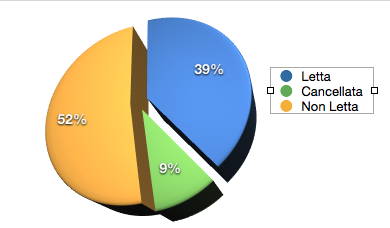
\includegraphics[scale=0.75]{img/statistica.png}
\caption{Statistica Mail}
\label{fig:statistica}
\end{figure}
Tali informazioni ci aiutano dunque a capire quanto importante e richiesto potrà essere un software di tale livello.